\addtocontents{toc}{\setcounter{tocdepth}{2}}
\chapter{Differentiation}
\section{What Is Differentiation?}

\textbf{None of this section on what differentiation is has to be known for the exam (except for the notation), though it's incredibly useful to know.}

\subsection{Understanding Rate of Change}
To measure how much something has changed, the difference can be found. For example, look at the following graph of the EUR/USD price from January to December 2019.

\begin{figure}[h!]
	\centering
	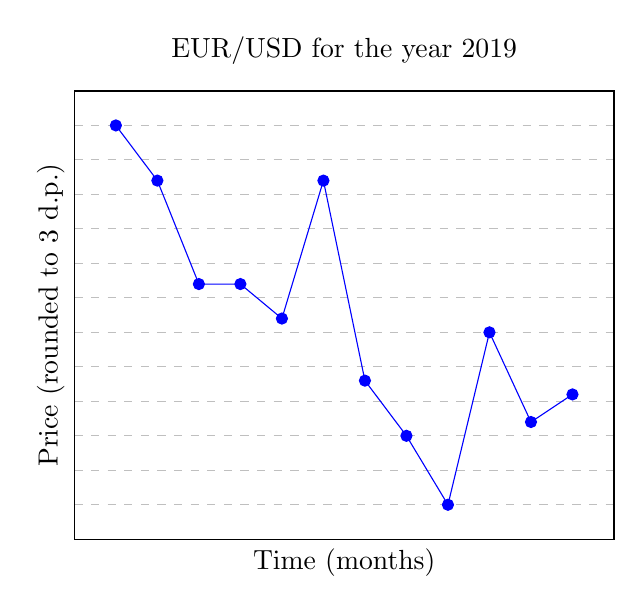
\begin{tikzpicture}
	\begin{axis}
	[
		title={EUR/USD for the year 2019},
		xlabel={Time (months)},
		ylabel={Price (rounded to 3 d.p.)},
		xmin=0,
		xmax=13,
		xtick={0,1,...,12},
		xticklabels={ ,Jan, Feb, Mar, Apr, May, Jun, Jul, Aug, Sep, Oct, Nov, Dec},
		ymin=1.085,
		ymax=1.150,
		ytick={1.085,1.090,...,1.145},
		x tick label style= {rotate=45, anchor=east},
		ymajorgrids=true,
		grid style=dashed,
		/pgf/number format/precision=3,
	]
		\addplot
		[
			color=blue,
			mark=*,
		] coordinates
		{
			(1,1.145) (2,1.137) (3,1.122) (4,1.122) (5,1.117) (6,1.137) (7,1.108) (8,1.100) (9,1.090) (10,1.115) (11,1.102) (12,1.106)
		};
	\end{axis}
	\end{tikzpicture}
	\caption{The EUR/USD course for January to December in 2019, rounded to 3 decimal places.}
	\label{fig:EURUSD}
\end{figure}

The change of the graph between December and January is the difference in their values. The exact values of those months are $1.145$ and $1.106$, so
\begin{align*}
	\text{difference in price} &= 1.145 - 1.106\\
	&=0.039\text{.}
\end{align*}

The rate of change is how quickly something changes, or in other words, the change that is experienced over time. The rate of change between January and December would be found by dividing the change by the time taken.

\begin{align*}
	\frac{\text{difference in price}}{\text{difference in time}} &=\frac{1.145-1.106}{12-1}\\[0.75em]
	&=\frac{0.039}{11} \approx 3.55\times10^{-3}
\end{align*}

More generally, the rate of change between any $x$ and $y$ is the difference in $y$ over the difference in $x$.
\begin{align*}
\text{rate of change} &= \frac{\text{difference in $y$}}{\text{difference in $x$}}
\end{align*}

\subsection{Paradox of the Instantaneous Rate of Change}
Suppose we graph the distance over time of a quick vehicle. For reasons that'll become more clear later on, the symbol $s$ is used for displacement instead of distance. This graph just so happens to be the graph of $d=t^2$, how convenient!

\begin{figure}[h!]
	\centering
	\begin{tikzpicture}
		\begin{axis}
		[
			restrict y to domain=0:25,
			restrict x to domain=0:5,
			xlabel=$t (s)$,
			ylabel=$d (m)$,
			xmin=0,
			xmax=5,
			xtick={0,1,...,4},
			ymin=0,
			ymax=17,
			ytick={0,2,...,16},
			axis lines=center,
			smooth,
			samples=50
		]
		\addplot [color=black,mark=none] {x^2};
		\end{axis}
	\end{tikzpicture}
	\caption{Displacement ($s$) in metres over time ($t$) in seconds.}
	\label{POIexample}
\end{figure}

The vehicle starts slowly and quickly begins to travel faster and faster. It would be very helpful to know how quick the car is going at a time of, say, 3 seconds. In other words, it would be helpful to know its instantaneous rate of change at 3 seconds (remember, rate of change is the change in value over time, in this case it's the change in displacement over time, the velocity).

The problem is that there is no such thing as "instantaneous" rate of change. To have a rate of change, there must be a time that has elapsed. That's not very helpful though, there must be a way to find out how quick the car is going --- its velocity (symbol $v$) --- at in a moment in time.

The solution to this is to decrease the change in time that's being used until it's nearly $0$, as close to $0$ as you could get. By coming closer and closer to 0, a certain value is approached. Let's try using a change in time of 3.1 and 3.01 and see what happens.

\begin{align*}
	v&=\frac{\text{difference in $d$}}{\text{difference in $t$}} & v&=\frac{\text{difference in $d$}}{\text{difference in $t$}}\\[0.75em]
	v &= \frac{3.1^2 - 3^2}{3.1-3} & v &= \frac{3.01^2 - 3^2}{3.01-3}\\[0.75em]
	v &= \frac{9.61-9}{3.1-3} & v &= \frac{9.0601-9}{3.01-3}\\
	&= 6.1 & &= 6.01
\end{align*}

As you can see, a value of $6$ is approached whenever a smaller value for the change in time is taken. As previously said, there is no such thing as instantaneous change, but instead the best approximation can be calculated. In this case, the best approximation for the rate of change can be concluded to be $6$.

That is what the derivative is. The best approximation for the rate of change.

Whenever the difference in the values approaches $0$, the symbol $d$ can be used, so more generally you can write for any $x$ and $y$,
\begin{equation}
	\text{rate of change} = \text{derivative} = \frac{dy}{dx}\text{.}
\end{equation}

\subsection{Notation}
When an equation (such as $d=t^2$ above) is differentiated, it is done with respect to one variable. Usually, equations are in the form $y=x$ where there might be lots on the $x$ side, but little on the $y$ side. When such an equation is differentiated, it is said to have been done ``with respect to x". The above example was differentiated with respect to $t$.

There are numerous ways of writing the derivative, each having a good use in different fields. In maths, two ways of writing the derivative are used: the one used by Leibniz, one of the independent discoverers of calculus, and the one used by Lagrange.

\subsubsection{Leibniz's Notation}
Leibniz notation is actually the one that has been used so far. The derivative of two variables $x$ and $y$ can be written as $\frac{dy}{dx}$ and is read out ``the derivative of $y$ with respect to $x$.
\subsection{Lagrange's Notation}
However, sometimes a function has to be differentiated. For example, the derivative of $f(x) = 6x^3$ is $18x^2$, but how is that written? A prime mark is added between the $f$ and $x$, and it is read as ``the derivative evaluated at $x$".
\begin{align*}
	f(x) &= 6x^3\\
	f'(x) &= 18x^2
\end{align*}


\addtocontents{toc}{\setcounter{tocdepth}{1}}
\section{A Shortcut to Differentiate}
Doing the above is very tedious, so luckily there is a shortcut that can be taken! Multiply the coefficient of the variable by the power, and subtract $1$ from the power. More formally,
\begin{align*}
	f(x) &= x^n\\
	f'(x) &= nx^{n-1}
\end{align*}

This is called the ``power rule".

Before power rule can be applied, however, the expression has to be rearranged so that each term is in the form $ax^n$. Look at the following and see how before the derivative is found the expression is rewritten.

\subsection{Examples}
Note that it's not required to continue to simplify after the derivative is found, however it might be helpful in more complex questions.

\begin{enumerate}
	\item
	\begin{align*}
		f(x) &= 5x^5\\
		f'(x) &= 25x^4
	\end{align*}
	\item
	\begin{align*}
		f(x) &= \frac{2}{x}\\
		&= x^{-2}\\
		f'(x) &= -2x^{-3}\\
		&= \frac{-2}{x^3}
	\end{align*}
	\item 
	\begin{align*}
		f(x) &= \frac{3}{\sqrt[4]{x^2}}\\
		&= \frac{3}{x^{\frac{2}{4}}}\\
		&= 3x^{-\frac{2}{4}}\\
		f'(x) &= -\frac{14}{4}x^{-\frac{6}{4}}\\[0.5em]
		&= \frac{-\frac{14}{4}}{x^{\frac{6}{4}}}\\[0.5em]
		&= \frac{-\frac{14}{4}}{\sqrt[4]{x^6}}
	\end{align*}
	\item
	\begin{align*}
		f(x)&=(x-3)(x+2)\\
		f(x)&=x^2-x-6\\
		f'(x)&=2x-1
	\end{align*}
	\item
	\begin{align*}
		f(x) &= \sqrt(x) \left(x^3 + \sqrt(x) \right)\\
		&= x^{\frac{1}{2}} \left(x^3+x^{\frac{1}{2}}\right)\\
		&= x^{\frac{7}{2}} + x\\
		f'(x) &= \frac{7}{2}x^{\frac{5}{2}}+1\\
		&= \frac{7}{2} \sqrt{x^5} + 1\\
		&= \frac{7 \sqrt{x^5}}{2} + 1
	\end{align*}
	\item
	\begin{align*}
		f(x) &= \frac{x^2 - 2x + 1}{\sqrt{x}}\\
		&= \frac{x^2 - 2x + 1}{x^{\frac{1}{2}}}\\
		&= \frac{x^2}{x^{\frac{1}{2}}} - \frac{2x}{x^{\frac{1}{2}}} + \frac{1}{x^{\frac{1}{2}}}\\
		&= x^{\frac{3}{2}} - 2x^{\frac{1}{2}} + x^{-\frac{1}{2}}\\
		f'(x) &= \frac{3}{2}x^{\frac{1}{2}} - x^{-\frac{1}{2}} - \frac{1}{2}x^{-\frac{3}{2}}\\
		&= \frac{3\sqrt{x}}{2} - \frac{1}{\sqrt{x}} - \frac{1}{2\sqrt{x^3}}
	\end{align*}
\end{enumerate}


\section{Gradient and Equation of a Tangent to a Curve}
\subsection{Explanation}
\textbf{Again, you aren't expected to explain this, but it's incredibly useful to understand what's happening.} You can skip to the examples at page \pageref{sec:derivativeExamples}.

Suppose there's a curve $y=(x-1)^2$, as shown in figure \ref{fig:gradientBasicExample}. How could you find gradient of the curve at, say, $x=3$?

\begin{figure}[h!]
	\centering
	\begin{tikzpicture}
		\begin{axis}
		[
			restrict y to domain=0:25,
			restrict x to domain=0:5,
			xlabel=$x$,
			ylabel=$y$,
			xmin=0,
			xmax=6,
			xtick={0,1,...,5},
			ymin=0,
			ymax=17,
			ytick={0,2,...,16},
			axis lines=center,
			smooth,
			samples=50
		]
			\addplot [color=black,mark=none] {(x-1)^2};
		\end{axis}
	\end{tikzpicture}
	\caption{Graph of $y=(x-1)^2$.}
	\label{fig:gradientBasicExample}
\end{figure}

Well, by definition, you need to have a change in $x$ to find the gradient. See what happens when values of $0.1$ and $0.01$ are used as changes in $x$.
\begin{align*}
	m &= \frac{y_2 - y_1}{x_2 - x_1} & m &= \frac{y_2 - y_1}{x_2 - x_1}\\
	&= \frac{(3.1-1)^2 - (3-1)^2}{3.1-3} & &= \frac{(3.01-1)^2 - (3-1)^2}{3.01-3}\\
	&= \frac{4.41 - 4}{3.1-3} & &= \frac{4.0401 - 4}{3.01-3}\\
	&= \frac{0.41}{0.1} & &= \frac{0.0401}{0.01}\\
	&= 4.1\dots & &= 4.01\dots
\end{align*}

Again, a value of $4$ is approached every time a smaller change in x is used. This might seem familiar if you've read the section on rate of change. The gradient as it approaches $0$ is the derivative.
\begin{equation*}
	m = \frac{y_2 - y_1}{x_2 - x_1} = \frac{dy}{dx}
\end{equation*}

So to apply that to the example above, what is the gradient at $x=3$?
\begin{align*}
	m &= \frac{dy}{dx}\\
	y &= (x-1)^2\\
	&= x^2-2x+1\\
	\frac{dy}{dx} &= 2x-2
\end{align*}
Sub $x=3$ into $2x-2$:
\begin{align*}
	&2(3)-2\\
	&=6-2\\
	&=4
\end{align*}

This is actually already half of the work required to find the tangent to the curve at $x=3$. Remember, a tangent to a curve is a line that touches a curve at only a single point. To find the equation of any line, $y-b=m(x-a)$ can be used. The gradient has already been found, and the point is given in the question, though the $y$ coordinate has to be found by substituting the given $x$ into the question again.

So for $x=3$, the gradient is $4$. $x=3$ is given, so it can be substituted into $y=(x-1)^2$.
\begin{align*}
	y&=(3-1)^2\\
	&=2^2\\
	&=4
\end{align*}
\textit{It is a coincidence} that the original equation gives the same as the derivative; this only happens in this equation at point $x=3$.

Substituting $m=4$ and $(3,4)$ into $y-b=m(x-a)$ gives the equation of the tangent.
\begin{align*}
	y-4&=4(x-3)\\
	y&=4x-12+4\\
	y&=4x-8
\end{align*}

\begin{figure}[h!]
	\centering
	\begin{tikzpicture}
		\begin{axis}
		[
			restrict y to domain=0:25,
			restrict x to domain=0:5,
			xlabel=$x$,
			ylabel=$y$,
			xmin=0,
			xmax=6,
			xtick={0,1,...,5},
			ymin=0,
			ymax=17,
			ytick={0,2,...,16},
			axis lines=center,
			smooth,
			samples=50
		]
			\addplot [color=black,mark=none] {(x-1)^2};
			\addplot [color=blue, mark=none] {4*x-8};
		\end{axis}
	\end{tikzpicture}
	\caption{The tangent at $x=3$ of $y=(x-1)^2$ in blue.}
	\label{fig:gradientFinishedExample}
\end{figure}

Figure \ref{fig:gradientFinishedExample} shows what the tangent actually looks like.


\section{Examples of Rate of Change \& Tangent of a Curve Questions}
\label{sec:derivativeExamples}
\subsection{Rate of Change}
Find the rate of change of $f(x) = x^-1$ when $x=4$.
\begin{align*}
	f(x) &= x^{-1}\\
	f'(x) &= -x^{-2}\\
	&= -\frac{1}{x^2}\\
	f'(4) &= -\frac{1}{4^2}\\
	&= -\frac{1}{16}
\end{align*}

\subsection{Tangent of a Curve}
Find the equation of the tangent of the curve of $y=-\left(\frac{x}{2}\right)^3+3x$ at $x=2$.
\begin{align*}
	y &= -\left(\frac{x}{2}\right)^3+3x\\
	&= -\left(\frac{x^3}{8}\right)+3x\\
	&= -\frac{1}{8}x^3+3x\\[1.5em]
	m&=\frac{dy}{dx}\\
	\frac{dy}{dx} &= -\frac{3}{8}x^2+3
\end{align*}
Substitute $x=2$ into $\frac{dy}{dx}$ to find the gradient.
\begin{align*}
	m &= -\frac{3}{8} \cdot 2^2+3\\
	&=-\frac{3}{8} \cdot 4 + 3\\
	&=-\frac{12}{8} + 3\\
	&=\frac{24}{8}\\
	&=\frac{3}{2}
\end{align*}
Substitute $x=2$ into the initial equation to get the $y$-coordinate.
\begin{align*}
	y&=-\left(\frac{x}{2}\right)^3+3x\\
	&=-\left(\frac{2}{2}\right)^3+3x\\
	&=-1^3 + 3 \cdot 2\\
	&=-1 + 6\\
	&=5
\end{align*}
Substitute $m=\frac{3}{2}$ and $(2,5)$ into $y-b=m(x-a)$.
\begin{align*}
	y-b&=m(x-a)\\
	y-5&=\frac{3}{2}\left(x-2\right)\\
	y&=\frac{3}{2}x-3+5\\
	y&=\frac{3}{2}x-+2
\end{align*}


\section{Graph of the Derivative}
There is a nice shortcut for sketching the graph of the derivative:

\begin{itemize}
	\item while the function is increasing, the derivative is in the positive $y$;
	\item while the function is decreasing, the derivative is in the negative $y$;
	\item while the function is stationary, the derivative $y=0$ --- in other words, \textit{the stationary points become roots.}
\end{itemize}

The graph of the derivative doesn't need to be perfect, as long as the general shape is correct, and the roots are labelled.

It's easier to show how it works, rather than to explain, see figure \ref{fig:graphOfDerivative}.

\begin{figure}[h!]
	\centering
	\begin{subfigure}{0.8\linewidth}
		\begin{tikzpicture}[cmark/.style={label={[anchor=center]:\pgfuseplotmark{#1}}}]
			\begin{axis}
			[
				restrict y to domain=0:10,
				restrict x to domain=-10:2,
				xlabel=$x$,
				ylabel=$y$,
				xmin=-3,
				xmax=2,
				xtick={-3,-2,...,1},
				ymin=-5,
				ymax=5,
				ytick={-5,-4,...,4},
				axis lines=center,
				smooth,
				samples=50,
				scale=1.6
			]
				\addplot [] {2*x^4+8*x^3+7*x^2-2*x+1};
				\coordinate
				[
					label=above:{$(-1,4)$},
					black,
					cmark=*,
				] (a) at (-1,4);
				\coordinate
				[
					label=right:{$\left(-\frac{\sqrt{5}}{2},\frac{7}{8}\right)$},
					black,
					cmark=*,
				] (b) at (-2.118034,0.875); %Approximate negative root 5 over 2.
				\coordinate
				[
					label=right:{$\left(\frac{\sqrt{5}}{2},\frac{7}{8}\right)$},
					black,
					cmark=*,
				] (c) at (0.1180340,0.875); %Approximate root 5 over 2.
			\end{axis}
		\end{tikzpicture}
	\end{subfigure}
	\begin{subfigure}{0.8\linewidth}
		\begin{tikzpicture}[bmark/.style={label={[anchor=center, color=blue]:\pgfuseplotmark{#1}}}]
		\begin{axis}
		[
			restrict y to domain=-10:10,
			restrict x to domain=-10:2,
			xlabel=$x$,
			ylabel=$y$,
			xmin=-3,
			xmax=2,
			xtick={-3,-2,...,1},
			ymin=-5,
			ymax=5,
			ytick={-5,-4,...,4},
			axis lines=center,
			smooth,
			samples=50,
			scale=1.6
		]
			\addplot [color=blue] {8*x^3+24*x^2+14*x-2};
			\coordinate
			[
				label=above right:{$(-1,0)$},
				black,
				bmark=*,
			] (a) at (-1,0);
			\coordinate
			[
				label=above left:{$\left(-\frac{\sqrt{5}}{2},0\right)$},
				black,
				bmark=*,
			] (b) at (-2.118034,0); %Approximate negative root 5 over 2.
			\coordinate
			[
				label=above right:{$\left(\frac{\sqrt{5}}{2},0\right)$},
				black,
				bmark=*,
			] (c) at (0.1180340,0); %Approximate root 5 over 2.
		\end{axis}
		\end{tikzpicture}
	\end{subfigure}
	\caption{$f(x)$ in black along with the $f'(x)$ in blue}
	\label{fig:graphOfDerivative}
\end{figure}

\section{Increasing and Decreasing Functions}
As you can see from above, when a function is increasing, its derivative is positive; when a function is decreasing, its derivative is negative. In questions about when functions are increasing and decreasing, it's helpful to write either of the following:

\begin{itemize}
	\item If $\frac{dy}{dx}>0$ then a function is increasing.
	\item If $\frac{dy}{dx}<0$ then a function is decreasing.
\end{itemize}

\subsection{Examples}
\begin{enumerate}
	\item
	Find the interval for which the graph of $y=4x^2+5x+7$ is increasing.
	
	If $\frac{dy}{dx}>0$ then a function is increasing.
	\begin{align*}
		\frac{dy}{dx} &> 0\\
		8x+5&>0\\
		8x&>-5\\
		x&>-\frac{5}{8}
	\end{align*}
	
	\item
	Show that the function $f(x) = x^3-3x^2+3x-10$ is never decreasing.
	\begin{align*}
		f'(x) &= 3x^2-6x+3\\
		&= 3(x^2-2x+1)\\
		&= 3(x-1)(x-1)\\
		&= 3(x-1)^2
	\end{align*}
	Because $x$ is squared $f'(x)$ can never be negative, and since a function decreases when $f'(x) < 0$ it will never decrease.
\end{enumerate}


\section{Stationary Points}
From figure \ref{fig:graphOfDerivative} it can be seen that when $\frac{dy}{dx} = 0$ then the graph isn't increasing or decreasing, it is stationary. The points where the graph is stationary are called stationary points (abbr. SP). These stationary points can be turning points (abbr. t.p.), or points of inflection (as shown in figure \ref{fig:inflexion}).

\begin{figure}[h!]
	\centering
	\begin{subfigure}{0.4\linewidth}
		\begin{tikzpicture}[bmark/.style={label={[anchor=center, color=blue]:\pgfuseplotmark{#1}}}]
			\begin{axis}
			[
				restrict y to domain=-3:3,
				restrict x to domain=-3:3,
				xlabel=$x$,
				ylabel=$y$,
				axis equal,
				axis lines=center,
				smooth,
				scale=0.65
			]
			\pgfplotsset{ticks=none}
			\addplot [] {x^3};
			\coordinate
			[
				bmark=*,
			] (a) at (0,0);
			\end{axis}
		\end{tikzpicture}
		\caption{Increasing point of inflexion.}
	\end{subfigure}
	\begin{subfigure}{0.4\linewidth}
		\begin{tikzpicture}[bmark/.style={label={[anchor=center, color=blue]:\pgfuseplotmark{#1}}}]
			\begin{axis}
			[
				restrict y to domain=-3:3,
				restrict x to domain=-3:3,
				xlabel=$x$,
				ylabel=$y$,
				axis equal,
				axis lines=center,
				smooth,
				scale=0.65
			]
				\pgfplotsset{ticks=none}
				\addplot [] {-x^3};
				\coordinate
				[
					bmark=*,
				] (a) at (0,0);
			\end{axis}
		\end{tikzpicture}
		\caption{Decreasing point of inflexion.}
	\end{subfigure}
	\caption{Points of inflexion.}
	\label{fig:inflexion}
\end{figure}

A nature table has to be drawn to show whether the stationary point is a maximum or minimum turning point, or a point of increasing or decreasing inflexion. To construct a nature table, a value slightly above and slightly below the $x$ value of the graph are chosen and put into the derivative. If the result is positive, then the graph is increasing, if it's negative it's decreasing.

The following example will make this a little clearer.

\subsection{Example}
Find the stationary points the curve of function $f(x) = 2x^3-9x^2+12x$.

\begin{equation*}
	f'(x) = 6x^2-18x+12
\end{equation*}

Stationary points occur when $f'(x)=0$.
\begin{align*}
	0 &= 6x^2-18x+12\\
	&= 6(x^2-3x+2)\\
	&= 6(x-2)(x-1)
\end{align*}
\begin{align*}
	x&=2 & x&=1
\end{align*}

Coordinates of stationary points calculated above.
\begin{align*}
	f(1) &= 2(1)^3-9(1)^1+12(1) & f(2) &= 2(2)^3-9(2)^2+12(2)\\
	&= 2(1)-9(1)+12(1) & &= 2(8)-9(4)+12(2)\\
	&= 2-9+12 & &= 16-36+24\\
	&= 5 & &=4\\
	\therefore &(1,5) & \therefore &(2,4)
\end{align*}

\textbf{Nature tables}

When the values of $f'(0.9)$, $f'(1.1)$ (1 doesn't need to be calculated, that's been done already after all), etc. are calculated, their sign gets put in the table as follows.

\medskip

\begin{tabular}{r | c c c}
	$x=1$ & $0.9$ & $1.0$ & $1.1$\\
	\hline
	$f'(x)$ & + & 0 & -\\
	Shape & / & $^{\text{---}}$ & \textbackslash \\
\end{tabular}

\medskip

\begin{tabular}{r | c c c}
	$x=2$ & $1.9$ & $2.0$ & $2.1$\\
	\hline
	$f'(x)$ & - & 0 & +\\
	Shape & \textbackslash & $_{\text{---}}$ & / \\
\end{tabular}


\section{Curve Sketching}
To sketch a curve the following are required:
\begin{enumerate}
	\item $y$-intercept (when $x=0$),
	\item $x$-intercept, a.k.a. roots (when $y=0$),
	\item stationary points and the nature of them,
	\item what happens as the curve approaches $\infty$ and $-\infty$.
\end{enumerate}

To figure out the $4^{\text{th}}$ bullet point, substitute an absurdly high and low number into the expression for the curve, something like $10^{12}$ and $-10^{12}$.

\subsection{Example}
Sketch the graph of $y=x^3-3x^2$.

\medskip

The graph cuts the $y$-axis when $x=0$.
\begin{align*}
	y&=(0)^3-3(0)^2\\
	&=0-3(0)\\
	&= 0\\
	\therefore&(0,0)
\end{align*}

The graph cuts the $x$-axis when $y=0$.
\begin{align*}
	x^3-3x^2&=0\\
	x^2(x-3)&=0
\end{align*}
\begin{align*}
	x&=0 & x&=3\\
	\therefore&(0,0) & \therefore&(3,0)
\end{align*}

Stationary points occur when $\frac{dy}{dx} = 0$.
\begin{equation*}
	\frac{dy}{dx} = 3x^2-6x
\end{equation*}
\begin{align*}
	0 &= 3x^2-6x\\
	&=3x(x-2)
\end{align*}
\begin{align*}
	3x&=0 & x-2&=0\\
	x&=0 & x&=2
\end{align*}
\begin{align*}
	\text{When } x&=0\text{,} & \text{When } x&=2\text{,}\\
	y&=0\text{.} & y&=(2)^3-3(2)^2\\
	& & &=8-12\\
	& & &=-4\\
	\therefore\text{ stationary points occur at } &(0,0) & \text{and }&(2,-4)
\end{align*}

\textbf{Nature tables}

\medskip

\begin{tabular}{r | c c c}
	$x=0$ & $-0.1$ & $0.0$ & $0.1$\\
	\hline
	$f'(x)$ & + & 0 & -\\
	Shape & / & $^{\text{---}}$ & \textbackslash \\
\end{tabular}

\medskip

\begin{tabular}{r | c c c}
	$x=2$ & $1.9$ & $2.0$ & $2.1$\\
	\hline
	$f'(x)$ & - & 0 & +\\
	Shape & \textbackslash & $_{\text{---}}$ & / \\
\end{tabular}

\begin{align*}
	y &= (10^{12})^3 - 3(10^{12})^2 & y &= (-10^{12})^3 - 3(-10^{12})^2\\
	&= 10^{36} & &= -10^{36}
\end{align*}
As $x \rightarrow \infty$, $y$ stays positive. As $x \rightarrow -\infty$, $y$ stays negative.
\begin{figure}[h!]
	\centering
	\begin{tikzpicture}[bmark/.style={label={[anchor=center, color=blue]:\pgfuseplotmark{#1}}}]
		\begin{axis}
		[
			restrict y to domain=-10:10,
			restrict x to domain=-10:10,
			xlabel=$x$,
			ylabel=$y$,
			xmin=-2,
			xmax=5,
			xtick={-2,-1,...,4},
			ymin=-5,
			ymax=5,
			ytick={-5,-4,...,4},
			axis lines=center,
			smooth,
			scale=1.3,
		]
			\addplot [color=blue] {x^3-3*x^2};
			\coordinate
			[
				label=above:{$(0,0)$},
				bmark=*,
			] (a) at (0,0);
			\coordinate
			[
				label=below:{$(2,-4)$},
				bmark=*,
			] (b) at (2,-4);
			\coordinate
			[
				label=above right:{$(3,0)$},
				bmark=*,
			] (c) at (3,0); %Approximate root 5 over 2.
		\end{axis}
	\end{tikzpicture}
	\caption{The curve from the curve sketching example. It doesn't have to be as perfect as it is here, as long as the shape and coordinates are correct.}
	\label{fig:curveSketchingExample}
\end{figure}

\section{Optimisation}
Finding where a function is at its minimum or at its maximum can be helpful for many real-life situations, for example the stock market. You could look at a prediction of the stock market and draw the following conclusions from here. Consider this idealised stock in figure \ref{fig:simpleStock}. It's best to sell at year 2 Q1, and best to buy at Q3.
\begin{figure}[h!]
	\centering
	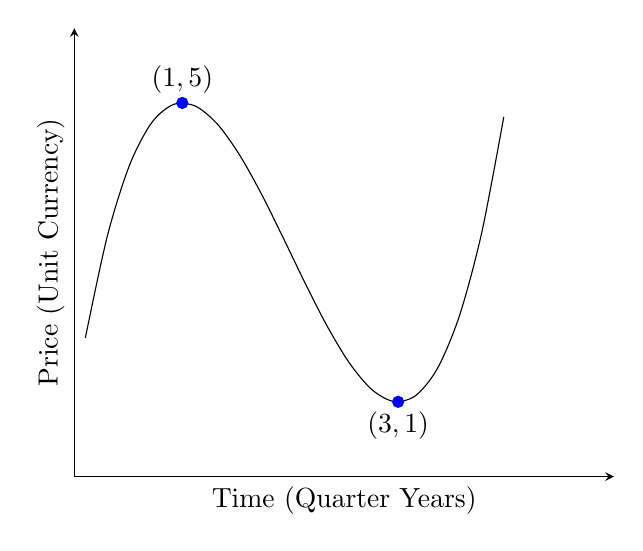
\begin{tikzpicture}[bmark/.style={label={[anchor=center, color=blue]:\pgfuseplotmark{#1}}}]
		\begin{axis}
		[
			restrict y to domain=0:10,
			restrict x to domain=0:4,
			xlabel=Time (Quarter Years),
			ylabel=Price (Unit Currency),
			xmin=0,
			xmax=5,
			xtick={0,1,...,4},
			xticklabels={Y1Q4,Y2Q1,Q2,Q3,Q4},
			ymin=0,
			ymax=6,
			ytick={0,1,...,5},
			axis lines=left,
			smooth,
			samples=50,
		]
		\addplot [] {(x-1)^3-3*(x-1)^2+5};
		\coordinate
		[
			label=above:{$(1,5)$},
			bmark=*,
		] (a) at (1,5);
		\coordinate
		[
			label=below:{$(3,1)$},
			bmark=*,
		] (b) at (3,1);
		\end{axis}
	\end{tikzpicture}
	\caption{A simplified stock.}
	\label{fig:simpleStock}
\end{figure}

As these ``best times to buy/sell" occur at stationary points, it's easy to find out what they are from an equation.

It's important to also consider the domain, since these are real-life examples. For example, that stock market graph might be continuing into an even lower value, but only that time frame might be of interest. Another example would be a geometric shape. Almost always the result cannot be negative.

Additionally, exam questions will often ask to show how the equation is derived. If you have no idea how to do that, just skip to the optimisation part to get at least a couple marks.

\subsection{Example}
The volume of a glass display case is 500 $cm^3$. The length of the base is $x$. The case is a bottom-less, square-based rectangular prism.
\begin{enumerate}
	\item Show that the area of the case is $A(x)=x^2+\frac{2000}{x}$.
	\item Find the dimensions of the case that minimises the use of glass, and calculate this minimum area.
\end{enumerate}

\bigskip

\begin{enumerate}
	\item
	The total area is the area on the top added to the area of the four sides combined. Since base is a square and has length $x$, an expression can be written (with variable $h$ for height).
	\begin{equation*}
		A(x) = x^2 + 4(hx)
	\end{equation*}
	
	To get rid of $h$, the equation for the volume of a cuboid can be used.
	\begin{align*}
		V &= x y z\\
		500 &= h x^2\\
		h &= \frac{500}{x^2}
	\end{align*}
	
	Substitute $h = \frac{500}{x^2}$ into $A(x) = x^2 + 4(hx)$.
	\begin{align*}
		A(x) &= x^2 + 4\left(x \cdot \frac{500}{x^2}\right)\\
		&= x^2 + 4\left(\frac{500x}{x^2}\right)\\
		&= x^2 + 4\left(\frac{500}{x}\right)\\
		&= x^2 + \frac{2000}{x}
	\end{align*}
	
	\item 
	To find the minimum area, the minimum turning point must be found.
	\begin{align*}
		A(x) &= x^2+2000x^{-1}\\
		A'(x) &= 2x-2000x^{-2}\\
		&= 2x-\frac{2000}{x^2}
	\end{align*}
	Since stationary points occur when $A'(x)=0$,
	\begin{align*}
		0 &= 2x-\frac{2000}{x^2}\\
		2x &= \frac{2000}{x^2}\\
		2x^3 &= 2000\\
		x^3 &= 1000\\
		x &= \sqrt[3]{1000}\\
		x &= 10
	\end{align*}
	
	To confirm that this is a minimum turning point:
	
	\textbf{Nature tables}
	
	\medskip
	
	\begin{tabular}{r | c c c}
		$x=10$ & $9.9$ & $10.0$ & $10.1$\\
		\hline
		$A'(x)$ & - & 0 & +\\
		Shape & \textbackslash & $_{\text{---}}$ & / \\
	\end{tabular}

	Therefore, a minimum turning point occurs at $x=10$.
	
	Work out the height:
	\begin{align*}
		h = \frac{500}{x^2}\\
		&= \frac{500}{10^2}\\
		&= 5
	\end{align*}
	
	Work out the area:
	\begin{align*}
		A(x) &= x^2+\frac{2000}{x}\\
		A(10) &= 10^2+\frac{2000}{10}\\
		&= 100+200\\
		&= 300\text{ cm}^3\text{.}
	\end{align*}
	
	Dimensions: 10 $\times$ 10 $\times$ 5 cm.
\end{enumerate}
